\documentclass[11pt,a4paper]{article}
\usepackage{mathtools}
\usepackage{graphicx}


\title{INF1060 - OS}
\author{Veronika Heimsbakk \\ 
veronahe@student.matnat.uio.no}
\begin{document}

\maketitle{}
\tableofcontents
\newpage{}

\section{Introduction}
INF1060 - Introduction to data communication and operative systems, is a course at the Department of Informatics at the University of Oslo. This is some notes about the OS part of the course. This document are more or less a copycat summary of the course book and the lecture slides. Mainly used for repetition for the exam.

\section{What is an operating system?}
The operating system is the most fundamental piece of software and runs in \textbf{kernel mode}. The rest of the software runs in \textbf{user mode}, in which only a subset of the machine instructions is available. 

\subsection{Computer hardware}
An OS is tied to the hardware on the computer it runs on. 

\subsubsection{Processors}
The CPU is the "brain" of the computer. The basis cycle of every CPU is to fetch the first instruction from memory, decode it to determine its type and operands, execute it, and then fetch, decode and execute subsequent instructions. This is repeated until the program is finished. All CPUs contains registers to hold key variables and temporary results. In addition to registers, most computers have several special registers that are visible to the user. One of these is the \textbf{program counter}, which contains the memory address of the next instruction to be fetched. Another one is the \textbf{stack pointer} which points to the top of the current stack in memory. Yet another one is the \textbf{Program Status Word (PSW)}. This contains the condition code bits, which are set by comparison instructions, the CPU priority, the mode (user or kernel), and various other control bits. The PSW plays and important role in the system calls and I/O.

\paragraph{Pipeline and Superscalar}
Many modern CPUs uses a \textbf{pipeline}. This makes it possible to have separate fetch, decode and execute units. Even more advanced that pipelines is a \textbf{superscalar} CPU. Here two or more instructions are fetched at once, decoded and dumped into a holding buffer until they can be executed. 

\paragraph{System Call}
Most CPUs have two modes. Kernel and user mode. When running in kernel mode, the CPU can execute every instruction in its instruction set and use every feature of the hardware. User programs run in  user mode, which permits only a subset of the instructions to be executed and a subset of the features to be accessed.  All instructions involving I/O and memory protection are disallowed in user mode. To obtain services from the OS, a user program must make a \textbf{system call}, which traps into the kernel and invokes the OS. The \texttt{TRAP} instruction switches from user mode to kernel mode and starts the OS. 

\subsubsection{Memory}
The second major component in any computer is the memory. The memory system is constructed as a hierarchy of layers. The top layers have higher speed, smaller capacity, and greater cost per bit than the lower ones, often by factors of a billion or more.

\begin{figure}[h!]
	\centering
		\includegraphics[width=300px]{memhi-01.png}
	\caption{A typical memory hierarchy.}
\end{figure}

The top layer consists of the registers internal to the CPU. 

Next comes the cache memory. Main memory is divided up into \textbf{cache lines}, typically 64 bytes, with addressed 0 to 63 in cache line 0, addresses 64 to 127 in cache line 1, and so on. Whenever there is a large resources that can be divided into pieces, caching is often invoked to improve performance. Cache is such a good idea that modern CPU's have two of them. The first \textbf{L1 cache} is always inside the CPU and usually feeds decoded instructions into the CPUs execution engine. \textbf{L2 cache} holds several megabytes of recently used memory words. The difference between L1 and L2 caches lies in the timing.

Main memory is usually called \textbf{Random Access Memory (RAM)}. All CPU requests that cannot be satisfied out of the cache go to the main memory. \textbf{Read Only Memory (ROM)} is programmed at the factory and cannot be changed afterwards. Some computers have the bootstrap in ROM.
Another kind of memory is CMOS, which is volatile. Many computers uses CMOS memory to hold the current time and date. The CMOS memory and the clock circuit that increments the time in it are powered by a small battery, so the time is correctly updated, even when the computer are unplugged. The CMOS memory may also hold configuration parameters, such as which disk to boot from.

\subsubsection{Disks}
Next in the hierarchy is the magnetic disk (hard disk). Disk storage is two orders of magnitude cheaper than RAM per bit and often two orders of magnitude larger as well. The only problem is that disks has low speed, due to the fact that they are magnetic.

A disk consists of one or more metal platters that rotate at 5400, 7200, or 10,800 rpm. A mechanical arm pivots over the platters from the corner. At any given arm position, each of the heads can read an annular region called a \textbf{track}. Together, all the tracks for a given arm position form a \textbf{cylinder}. Each track is divided into some number of sectors, typically 512 bytes per sector.

\subsubsection{Booting the Computer}
On the motherboard is a program called the system \textbf{Basic Input Output System (BIOS)}. The BIOS contains low-level I/O software, including procedures to read the keyboard, write to the screen, and do disk I/O, among other things. The BIOS determines the boot device by trying a list of devices stored in the CMOS memory.

\section{Processes}
All runnable software on the computer, sometimes including the OS, is organized into a number of processes. A process is just an instance of an executing program, including the current values of the program counter, registers and variables. Conceptually each process has its own virtual CPU. In reality, ofc, the CPU switches back and forth from process to process. This switching is called \textbf{multiprogramming}.

Processes that stay in the background to handle some activity such as e-mail, web pages, news and so on are called \textbf{daemons}.

\subsection{Process Creation}
There are four principal events that cause processes to be created:
\begin{enumerate}
\item{System initialization.}
\item{Execution of a process creation system call by a running process.}
\item{A user request to create a new process.}
\item{Initiation of a batch job.}
\end{enumerate}

Often a running process will issue system calls to create one or more new processes to help it do its job. In UNIX, there is only one system call to create a new process: \texttt{fork}. This call creates an exact clone of the calling process.

\subsection{Process Termination}
Usually due to one of the following conditions:
\begin{enumerate}
\item{Normal exit (voluntary).}
\item{Error exit (voluntary).}
\item{Fatal error (involuntary).}
\item{Killed by another process (involuntary).}
\end{enumerate}

\subsection{Process States}

\begin{enumerate}
\item{Running (actually using the CPU at that instant).}
\item{Ready (runnable; temporarily stopped to let another process run).}
\item{Blocked (unable to run until some external event happens).}
\end{enumerate}

\begin{figure}[h!]
	\centering
		\includegraphics[width=300px]{img/pro-01.png}
	\caption{Process states.}
\end{figure}

The first two states are similar. In both cases the process is willing to run, only in the second one, there is temporarily no CPU available for it. The third state is different because the process cannot run, even if the CPU has nothing else to do. When a process blocks, it does so because it cannot continue, typically because it is waiting for input that is not yet available.

\subsection{Scheduling}
If only one CPU is available, a choice has to be made which process to run next. The part of the OS that makes the choice  is called the \textbf{scheduler}, and the algorithm it uses is called the \textbf{scheduling algorithm.}

When the kernel mode manages threads, scheduling is usually done per thread, with little or no regard to which process the thread belongs. 

\subsubsection{When to Schedule}
When a new process is created, a decision needs to be made whether to run the parent process or the child process. A scheduling decision also needs to be made when a process exits. If no process is ready, a system-supplied idle process is normally run.
When an I/O interrupt occurs, a scheduling decision may be made. 

A \textbf{nonpreemptive} scheduling algorithm picks a process to run and then just lets it run until it blocks or until it voluntarily releases the CPU.

A \textbf{preemptive} scheduling algorithm picks a process and lets it run for maximum of some fixed time. Doing preemptive scheduling requires having a clock interrupt occur at the end of the time interval to give control of the CPU back to the scheduler.

\paragraph{Categories of Scheduling Algorithms}
\begin{enumerate}
\item{Batch.}
\item{Interactive.}
\item{Real time.}
\end{enumerate}

The batch algorithms are actually fairly general and often applicable to other situations as well. Interactive users, is preemptive essential to keep one process from hogging the CPU and denying service to the others. Servers also fall into this category, since they normally serve multiple users. Real-time constraints, preemptive is, oddly enough, sometimes not needed because the processes know that they may not run for long periods of time and usually do their work and block quickly.

\subsubsection{Scheduling in Batch Systems}

\paragraph{First-Come First-Serve}
The simplest nonpreemptive algorithm is maybe \textbf{first-come first-served}. Processes are assigned to the CPU in the order they request it. A single queue of ready processes. When the first job enters the system, it is started immediately and allowed to run as long as it wants to. As other jobs come in, they are put onto the end of the queue. With this algorithm, a single linked list keeps track of all ready processes.

\paragraph{Shortest Job First}
\begin{figure}[h!]
	\centering
		\includegraphics[width=300px]{img/short-01.png}
	\caption{An example of shortest job first scheduling. (a) Running four jobs in original order. (b) Running them in shortest job first order.}
\end{figure}

When several equally important jobs are sitting in the input queue waiting to be started, the scheduler picks the \textbf{shortest job first}. This algorithm is only optimal when all the jobs are available simultaneously.

\paragraph{Shortest Remaining Time Next}
A preemptive version of of shortest job first.  The scheduler always choses the process whose remaining run time is the shortest. Run time hat to be known in advance. If the new job needs less time to finish than the current process, the current process is suspended and the new job started. 

\subsubsection{Scheduling in Interactive Systems}
These algorithms are common on personal computers, servers and other.

\paragraph{Round-Robin Scheduling}
This is the most widely used algorithm. Each process is assigned a time interval, called its \textbf{quantum}, during which it is allowed to run. If the process is still running at the end of the quantum, the CPU is preempted and given to another process. If the process has blocked or finished before the quantum has elapsed, the CPU switching is done when the process blocks.

The issue about this algorithm is the length of the quantum. Switching from one process to another requires a certain amount of time for doing the administration. This switching is called \textbf{process switch} or \textbf{context switch}, and it takes 1 msec, including switching memory maps, flushing and reloading the cache, etc. 

Suppose the quantum is set to 4 msec. With these parameters, the CPU have to spend 1 msec on switching. That is 20\% of CPU time wasted on administrative overhead. To improve CPU efficiency, we may set the quantum to 100 msec, and the waste time is only 1\%. But here is the problem -- if 50 short jobs come in on an e.g. server. The first job may start right away, and the second one may not start until 100 msec later and so on. This created delay for the user.  With a short quantum they would have gotten better service. 

Another factor is that if the quantum us set longer than the mean CPU burst, preemption will not happen very often. Instead, most processes will perform a blocking operation before the quantum runs out, causing process switch.

\subparagraph{Summary} 
Setting the quantum too short causes too many process switches and lowers the CPU efficiency, but setting it too long may cause poor response to short interactive requests. A quantum around 20-50 msec is often a reasonable compromise.

\paragraph{Priority Scheduling}
Round-robin scheduling makes the implicit assumption that all processes are equally important. The need to take external factors into account leads to \textbf{priority scheduling}. Basic idea: each process is assigned a priority, and the runnable process with the highest priority is allowed to run. 

For example, a daemon process sending electronic mail in the background should be assigned a lower priority than a process displaying video film on the screen. To prevent high-priority processes from running indefinitely, the scheduler may decrease the priority of the current running process at each clock tick. If this causes its priority to drop below that of the next highest process, a process switch occurs. Alternatively, each process may be assigned a maximum time quantum that it is allowed to run.

\begin{figure}[h!]
	\centering
		\includegraphics[width=300px]{img/pri-01.png}
	\caption{A scheduling algorithm with four priority classes.}
\end{figure}

\paragraph{Shortest Process Next}
Similar to shortest job first. Interactive processes generally follows the pattern of wait for command, execute command, wait for command and so on. If we regard the execution of each command as a separate "job", then we could minimize overall response time by running the shortest one first. The problem is figuring out which of the current runnable processes is the shortest one. 

\paragraph{Lottery Scheduling}
Basic idea: give process lottery tickets for various system resources, such as CPU time. Whenever a scheduling decision has to be made, a lottery ticket is chosen random, and the process holding that ticket gets the resource. When applied to CPU scheduling, the system might hold a lottery 50 times a second, with each winning getting 20 msec of CPU time as a prize. 

More important processes can be given extra tickets, to increase their odds of winning.

In contrast to a priority scheduler, where it is very hard to state what having a priority of 40 actually means, here the rule is: a process holding a fraction $f$ of the tickets will get about fraction $f$ of the resource in question.

If a new process shows up and is granted some tickets, at the very next lottery it will have a chance of winning in proportion to the number of tickets it holds. 

Cooperating processes may exchange tickets if they wish.

\section{Memory Management}
\subsection{Address Spaces}
An address space is the set of addresses that a process can use to address memory. Each process has its own address space, independent of those belonging to other processes. 

Address spaced do not have to be numeric. The set of \textit{.com} Internet domains is also an address space.

\subsubsection{Base and Limit Registers}
The simplest version used a simple version of \textbf{dynamic relocation}. What it does is map each process' address space onto a different part of physical memory in a simple way. Equip each CPU with two special hardware registers, called \textbf{base} and \textbf{limit} registers. When these are used, programs are loaded into consecutive memory locations wherever there is room and without relocation during loading. When a process is run, the base register is loaded with the physical address where its program begins in memory, and the limit register is loaded with the length of the program. 

A disadvantage of relocation using base and limit registers is the need to preform an addition and a comparison on every memory reference.

\subsection{Swapping}
Two general approaches to dealing with memory overload have been developed over the years. The simplest strategy, called \textbf{swapping}, consists of bringing in each process in its entirety, running it for a while, then putting it back on the disk. The other strategy, called \textbf{virtual memory}, allows programs to run even when they are only partially in main memory.

\begin{figure}[h!]
	\centering
		\includegraphics[width=300px]{img/memall-01.png}
	\caption{Operation of swapping system. The shaded areas are unused memory.}
\end{figure}

In Fig. 5 we see the swapping operation. Only process $A$ is in memory. Then process $B$ and $C$ are created or swapped in from disk. In Fig. 5(d) $A$ is swapped out to disk. Then $D$ appears, and $B$ goes out. $A$ finally comes in again. Since $A$ is now at a different location, addresses contained in it must be relocated, either by software when it is swapped in or by hardware during program execution. For example, base and limit registers. 

When swapping creates multiple holes in memory, it is possible to combine them all into one big one by moving all the processes downward as far as possible. This technique is known as \textbf{memory compaction}. It is usually not done because it requires a lot of CPU time.

\subsubsection{Memory Management with Bitmaps}
With bitmaps, memory is divided into allocation units as small as a few words and as large as several kilobytes. The smaller the allocation unit, the larger the bitmap.

However, with an allocation unit as small as 4 bytes, 32 bits of memory will require only 1 bit of the map. A memory of 32$n$ its will use $n$ map bits, so the bitmap will take up only 1/33 of memory. If the allocation unit is chosen large, the bitmap will be smaller, but appreciable memory may be wasted in the last unit of the process if the process size is not an exact multiple of the allocation unit.

The size of the bitmap depends only on the size of memory and the size of the allocation unit.

An argument against bitmap: it is a slow operation to search a bitmap of a given length.

\subsubsection{Memory Management with Linked Lists}
Another way of keeping track of memory is to maintain a linked list of allocated free memory segments, where a segment either contains a process or is an empty hole between two processes.

\begin{figure}[h!]
	\centering
		\includegraphics[width=300px]{img/memlink-01.png}
	\caption{Four neighbor combinations for the termination process, $X$.}
\end{figure}

In Fig. 6(a) updating the list requires replacing a P by H. In Fig. 6(b) and (c), two entries are coalesced into one, and the list becomes one entry shorter. In Fig. 6(d), three entries are merged and two items are removed from the list. Since the process table slot for the terminating process will normally point to the list entry for the process itself, it may be more convenient to have the list as a double linked list, rather than the single-linked list. This makes it easier to find the previous entry and to see if a merge is possible.

\paragraph{Allocation Algorithms}
When the processes and holes are kept on a list sorted by addresses, several algorithms may be used. Maybe the simplest one is \textbf{first fit}. The memory manager scans along the list of segments until it finds a hole that is big enough. The hole is then broken up into two pieces, one for the process and one for the unused memory. 

First fit is a fast algorithm because it searches as little as possible.

A minor variation of first fit is \textbf{next fit}. It works the same way as first fit, except that it keeps track of where it is whenever it finds a suitable hole. Next fit gives slightly worse performance than first fit.

Another one is \textbf{best fit}, this is widely used. Best fit searches the entire list, from beginning to end, and takes the smallest hole that is adequate. Rather than breaking up a big hole that might be needed later.

If a block of size 2 is needed, first fit will allocate the hole at 5, but best fit will allocate the hole at 18. Best fit is slower than first fit because it must search the entire list every time it is called. It also results in more wasted memory than first fit or next fit, because it tends to fill up memory with tiny, useless holes. First fit generates larger holes on the average.

With a hole list sorted by size, first fit and best fit are equally fast, and next fit is pointless. 

Yet another algorithm is \textbf{quick fit}, which maintains separate lists for some of the more common size requested. With quick fit, finding a hole of the required size is extremely fast, but it has the same disadvantage as all schemes that sort by hole size, namely, when a process terminates or is swapped out, finding its neighbors to see if a merge is possible is expensive.  

\subsection{Virtual Memory}
As a consequence of technology developments, there is a need to run programs that are too large to fit in memory, and there is certainly a need to have systems that can support multiple programs running simultaneously, each of which fits in memory but which collectively exceed memory. Swapping is not an attractive option, since a typical SATA disk has a peak transfer rate of at most 100 MB/sec, which means it takes at least 10 sec to swap out a 1GB program and another 10 sec to swap in a 1GB program.

The basic idea behind \textbf{virtual memory} is that each program has its own address space, which is broken up into chunks called \textbf{pages}. Each page is a contiguous range of addresses.

In a sense, virtual memory is a generalization of the base and limit register idea. With virtual memory, instead of having separate relocation for just the text and data segments, the entire address space can be mapped onto physical memory in fairly small units.

\subsubsection{Paging}
Addresses can be generated using indexing, base registers, segment registers and other ways.

\begin{figure}[h!]
	\centering
		\includegraphics[width=300px]{img/mmu-01.png}
	\caption{The position and function of the MMU. Here the MMU is shown as being a part of the CPU chip because it commonly is nowadays. However, logically it could be a separate chip and was in years gone by.}
\end{figure}

These program-generated addresses are called \textbf{virtual addresses} and form the \textbf{virtual address space}. When virtual memory is used, the virtual addresses do not go directly to the memory bus. Instead, they go to an \textbf{Memory Management Unit (MMU)} that maps the virtual addresses onto the physical memory addresses, as shown in Fig. 7.

The virtual address space is divided into fixed-size units called \textbf{pages}. The corresponding units in the physical memory are called \textbf{page frames}. The pages and page frames are generally the same in size. 

\begin{figure}[h!]
	\centering
		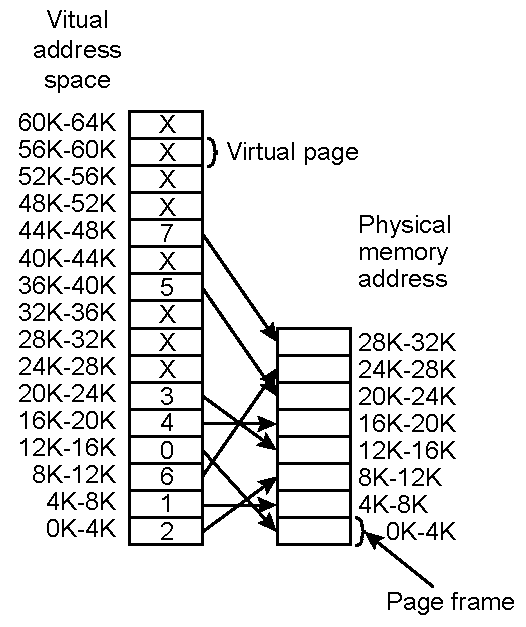
\includegraphics{img/page.pdf}
	\caption{The relation between virtual addresses and physical memory addresses is given by the page table. Every page begins on a multiple of 4096 and ends 4095 addresses higher, so 4K-8K really means 4096-8191.}
\end{figure}

The MMU notices that the page is unmapped (marked with X in Fig. 8) and causes the CPU to trap to the operating system. This trap is called a \textbf{page fault}. The OS picks a little-used page frame and writes its contents back to the disk. IT then fetches the page just referenced into the page frame just freed, changes the map, and restarts the trapped instruction.

\subsubsection{Page Tables}
In a simple implementation, the mapping of virtual addresses onto physical addresses can be summarized as follows: the virtual address is split into a virtual page number (high-order bits) and an offset (low-order bits). The virtual page number is used as an index to the page table to find the entry for that virtual page. From the page table entry, the page frame number is found. The page frame number is attached to the high-order end of the offset, replacing the virtual page number, to from a physical address that can be sent to memory. The purpose of the page table is to map virtual pages onto page frames.

\paragraph{Structure of a Page Table Entry}
Fig. 9 shows an example of a page table entry. The size varies from computer to computer.

\begin{figure}[h!]
	\centering
		\includegraphics[width=300px]{img/entry-01.png}
	\caption{A typical page table entry.}
\end{figure}

The most important field is the \textit{page frame number}. The goal of the page mapping is to output this value. Next to it we have the \textit{present/absent} bit. If this bit is 1, the entry is valid and can be used. If it is 0, the virtual page to which the entry belongs is not currently in memory. Accessing a page table entry with this bit set to 0 causes a page fault.
The \textit{protection} bits tell what kinds of access are permitted. In the simplest form, this field contains of one bit. 0 for read/write and 1 for read only. The \textit{modified and reference} bits keep track of page usage. If the page in it has been modified ("dirty"), it must be written back to the disk. If it has not been modified ("clean"), it can just be abandoned, since the disk copy is still valid. The last bit allows caching to be disabled for the page. Important for pages that map onto device registers rather than memory.

The page table holds only that information the hardware needs to translate a virtual address to a physical address.

\subsubsection{Page Replacement Algorithms}
\begin{table}[h!]
	\begin{center}
		\begin{tabular}{| l | l |}
		\hline
		\textbf{Algorithm} & \textbf{Comment} \\
		\hline
		Optimal & Not implementable, but useful as a benchmark.\\
		\hline
		Not Recently Used (NRU) & Very crude approximation of LRU. \\
		\hline
		First-In, First-Out (FIFO) & Might throw out important pages.\\
		\hline
		Second chance & Big improvement over FIFO.\\
		\hline
		Clock & Realistic.\\
		\hline
		Least Recently Used (LRU) & Excellent, but difficult to implement exactly.\\
		\hline
		Not Frequently Used (NFU) & Fairly crude approximation to LRU.\\
		\hline
		Aging & Efficient algorithm that approximates LRU well.\\
		\hline
		Working set & Somewhat expensive to implement.\\
		\hline
		WSClock & Good efficient algorithm.\\
		\hline
		\end{tabular}
	\end{center}
	\caption{Page replacement algorithms.}
\end{table}

The optimal algorithm evicts the page that will be referenced furthest in the future. Unfortunately, there is no way to determine which page this is, so in practice this algorithm cannot be used. 

The NRU algorithm divides pages into four classes depending on the state of the $R$ and $M$ bits. A random page from the lowest-numbered class is chosen. 

FIFO keeps track of the order in which pages were loaded into memory by keeping them in a linked list. Removing the oldest page then becomes trivial, but that page might still be in use. FIFO is a bad choice.

Second chance is a modification to FIFO that checks if a page is in use before removing it. If it is, the page is spared. 

Clock is simply a different implementation of second chance. It has the same performance properties, but takes a little less time to execute the algorithm. 

LRU is an excellent algorithm, but it cannot be implemented without special hardware. Basic LRU idea: when a page fault occurs, throw out the page that has been unused for the longest time.

NFU is a crude attempt to approximate LRU. It is not very good. However, aging is much better approximation to LRU and can be implemented efficiently. It is a good choice.

\section{File Systems}
\subsection{Files}
\textbf{Files} are logical units of information created by processes. A disk will usually contain thousands, or even millions of them. Information stored in files must be \textbf{persistent}.

\subsubsection{File Naming}
When a process creates a file, it gives the file a name. When the process terminates, the file continues to exist and can be accessed by other processes using its name. All current operative systems allow strings of one to eight letters. Many file systems support names as long as 255 characters. Some systems also distinguish between upper and lower case letters. A UNIX system can have all of the following as three distinct files: \textit{maria}, \textit{Maria}, \textit{MARIA}. In MS-DOS, all these names refer to the same file.

\subsubsection{File Types}
\textbf{Regular files} are the ones that contain user information. \textbf{Directories} are the system files for maintaining the structure of the file system. \textbf{Character special files} are related to input/output and used to model serial I/O devices, such as terminals, printers etc. \textbf{Block special files} are used to model disks. 

\subsection{Directories}
To keep track of files, file systems have \textbf{directories} or \textbf{folders}. These are often files themselves.

\subsubsection{Single-Level Directory System}
This is the simplest form of directory system. Having one directory containing all the files. 

\begin{figure}[h!]
	\centering
		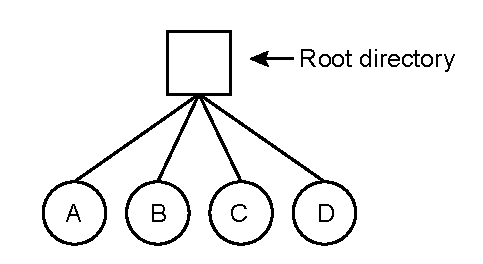
\includegraphics{img/single.pdf}
	\caption{A single-level directory system containing four files.}
\end{figure}

\subsubsection{Hierarchical Directory System}
If multiple users share a common file server, as is the case on many company networks, each user can have a private root directory for his or her own hierarchy. 

\begin{figure}[h!]
	\centering
		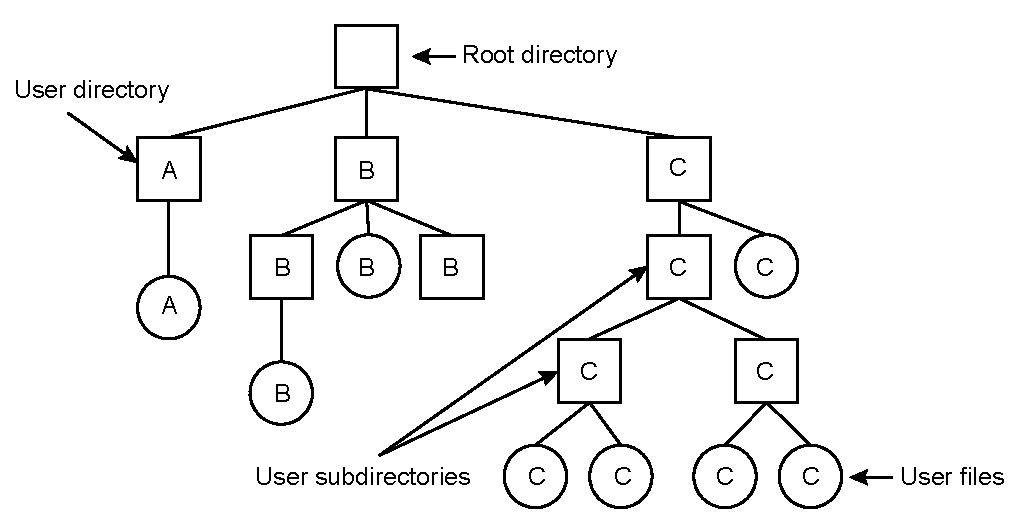
\includegraphics[width=\linewidth]{img/hir.pdf}
	\caption{A hierarchical directory system.}
\end{figure}

\subsubsection{Path Names}
There are two different methods that are commonly used. In the first method, each file is given an \textbf{absolute path name} consisting of the path from root directory to the file. Example: \textit{/usr/ast/mailbox}. Absolute path names always start at the root directory and are unique. In the UNIX system the components of the path are separated by /. In Windows the separator is \textbackslash.

The other kind is \textbf{relative path name}. This is used in conjunction with the concept of \textbf{working directory}. Example, if the current work directory is \textit{/usr/ast}, then the file whose absolute path is \textit{/usr/ast/mailbox} can be referenced simply as \textit{mailbox}.

\subsection{File System Implementation}
\subsubsection{File System Layout}
File systems are stored on disks. Sector 0 of the disk is called the \textbf{Master Boot Record (MBR)} and is used to boot the computer. The end of the MBR contains the partition table. This table gives the starting and ending addresses of each partition. When the computer is booted, the BIOS reads in and executes the MBR. The first thing the MBR program does is locate the active partition, read in its first block, called the \textbf{boot block}, and execute it. The program in the boot block loads the OS contained in that partition. 

Often the file system will contain some of the items shown in Fig. 12. 

\begin{figure}[h!]
	\centering
		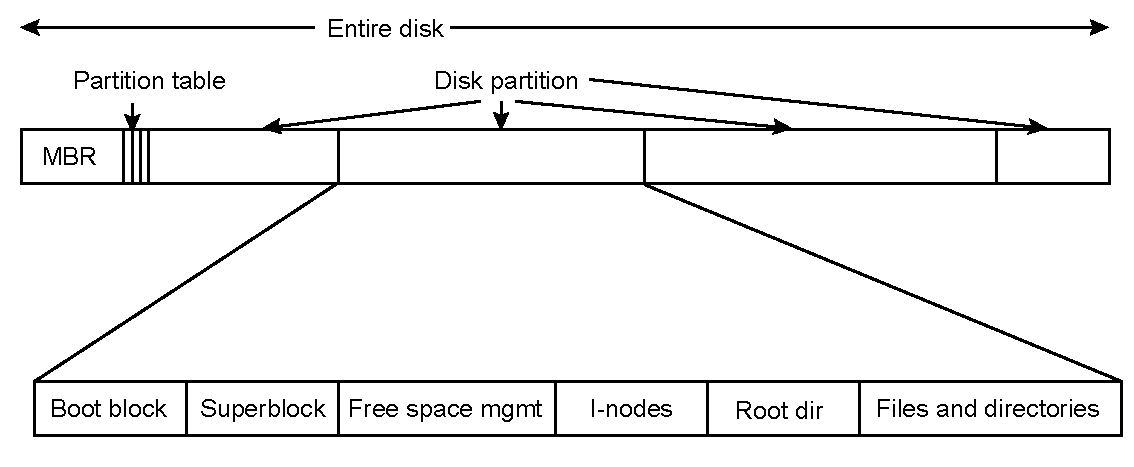
\includegraphics[width=\linewidth]{img/disk.pdf}
	\caption{A possible file system layout.}
\end{figure}

The first one is the \textbf{superblock}. It contains all the key parameters about the file system and is read into memory when the computer is booted or the file system is first touched. 
Next come information about free blocks in the file system, for example in the form of a bitmap or a list of pointers. This might be followed by the i-nodes, and array of data structures, one per file, telling about the file. After that might come the root directory, which contains the top of the file system tree. Finally, the remainder of the disk contains all the other directories and files.

\subsubsection{Implementing Files}
\paragraph{Contiguous Allocation}
The simplest allocation scheme is to store each file as a contiguous run of disk blocks. Thus on a disk with 1KB blocks, a 50KB file would be allocated 50 consecutive blocks. 
This has two significant advantages. First, it is simple to implement because keeping track of where a file's blocks are is reduced to remembering two numbers: the disk address of the first block and the number of blocks in the file. 
Second, the read performance is excellent because the entire file can be read from the disk in a single operation. Only one seek is needed. 

A significant drawback with this is that over time, the disk becomes fragmented.

This method is widely used on CD-ROMs.

\paragraph{Linked List Allocation}
The second method for storing files is to keep each one as a linked list of disk blocks. The first word of each block is used as a pointer to the next one. The rest of the block is for data. Unlike contiguous allocation, every disk block can be used in this method.

Although reading a file is straightforward, random access is extremely slow. Also the amount of data storage in a block is no longer a power of two, because the pointer takes up a few bytes. 

\paragraph{Linked List Allocation Using a Table in Memory}
Both disadvantages of the linked list allocation can be eliminated by taking the pointer word from each disk block and putting it in a table in memory. 

\begin{figure}[h!]
	\centering
		\includegraphics[width=300px]{img/table-01.png}
	\caption{Linked list allocation using file allocation table in main memory.}
\end{figure}

We have two files: $A$ an $B$. File $A$ uses disk blocks 4, 7, 2, 10 and 12, in that order. File $B$ uses disk blocks 6, 3, 11 and 14, in that order. Using table of Fig. 13 we can start with block 4 and follow the chain all the way to the end. The same can be done starting with block 6. Both chains are terminated with a special marker (e.g. $-1$) that is not a valid block number. Such a table in main memory is called \textbf{File Allocation Table (FAT)}.

The disadvantage of this method is that the entire table must be in memory all the time to make it work. With a 200GB disk and a 1KB block size, the table needs 200 million entries, one for each of the 200 million disk blocks. The FAT idea does not scale well to large disks.

\paragraph{I-nodes}
Our last method for keeping track of which blocks belong to which file is to associate with each file a data structure called an \textbf{i-node (index node)}, which lists the attributes and disk addresses of the file's blocks. A simple example is shown in Fig. 14.

\begin{figure}[h!]
	\centering
		\includegraphics[width=300px]{img/inode-01.png}
	\caption{An example i-node.}
\end{figure}

The big advantage of this scheme over linked files using an in-memory table is that the i-node need only to be in memory when the corresponding file is open. If each i-node occupies $n$ bytes and a maximum of $k$ files may be open at once, the total memory occupied by the array holding the i-nodes for the open files is only $kn$ bytes. 

\section{Disks}
The mechanic of disks consists of:
\begin{itemize}
\item{\textbf{Platters}: circular platters covered with magnetic material to provide nonvolatile storage of bits.}
\item{\textbf{Spindle}: of which the platters rotate around.}
\item{\textbf{Tracks}: concentric circles on a single platter.}
\item{\textbf{Disk headers}: read or alter the magnetism (bits) passing under it. The heads are attached to an arm enabling it to move across the platter surface.}
\item{\textbf{Cylinders}: corresponding tracks on the different platters are said to form a cylinder.}
\item{\textbf{Sectors}: segment of the track circle -- usually each contains 512 bytes -- separated by non-magnetic gaps. The gaps are often used to identify the beginning of a sector.}
\end{itemize}

The disk capacity depends on the number of platters, whether the platters uses one or both sides, number of tracks per surface and so on.

\subsection{Disk Access Time}
The disk retrieves data from the disk by position the head over the cylinder (track) on which block are located. It reads or writes the data block as the sectors are moved under the head when the platters rotate. 

The time between the moment issuing a disk request and the time the block is resident in memory is called \textbf{disk latency} or \textbf{disk access time}.

The access time may be summarized as follows: disk access time = seek time + rotational delay + transfer time + other delays

\paragraph{Seek Time} is the time to position the head. Time to move the head: $\alpha + \beta \sqrt{n}$, where $\alpha$ is the fixed overhead, $\beta$ is the seek time constant and $n$ the number of tracks.

\paragraph{Rotational Delay}is the time for the disk platters to rotate so the first of the required sectors are under the disk head. Average delay is 1/2 revolution.

\paragraph{Transfer Time} is the time for data to be read by the disk head. Transfer time is dependent on \textbf{data density} and \textbf{rotation speed}.

\paragraph{Other Delays} may be CPU time to issue and process I/O, contention for controller, contention for bus, contention for memory and so on.

\subsection{Data Scheduling}
\subsubsection{First-Come First-Serve (FCFS)}
FCFS serves the first arriving request first. It got long seeks and short response time for all.
\begin{figure}[h!]
	\centering
		\includegraphics[width=350px]{img/fcfs-01.png}
	\caption{An example with FCFS scheduling.}
\end{figure}

\subsubsection{Shortest Seek Time First (SSTF)}
SSTF serves closest request first. Shortest seek times, longer maximum response times -- may even lead to starvation.
\begin{figure}[h!]
	\centering
		\includegraphics[width=350px]{img/sstf-01.png}
	\caption{An example with SSTF scheduling.}
\end{figure}

\subsubsection{SCAN}
SCAN (elevator) moves head edge to edge and serves requests on the way. Bi-directional, compromise between response time and seek time optimizations. Several optimizations: C-SCAN, LOOK, C-LOOK, $\dots$
\begin{figure}[h!]
	\centering
		\includegraphics[width=350px]{img/scan-01.png}
	\caption{An example with SCAN scheduling.}
\end{figure}

\section{Input/Output}
\subsection{I/O Devices}
I/O devices can be roughly divided into two categories: \textbf{block devices} and \textbf{character devices}. A block device is one that stores information in fixed-size blocks, each one with its own address. Common block-sizes range from 512 bytes to 32,768 bytes. All transfers are in units of one or more blocks. Hard disks, CD-ROMs and USB sticks are block devices. 

A character device delivers or accepts a stream of characters, without regard to any block structure. It is not addressable and does not have an seek operation. Printers, network interfaces and mice can be seen as character devices. 

This classification scheme is not perfect, some devices do not fit in. Clocks, for example, are not block addressable. Nor do they generate or accept character streams. All they do is interrupts as well-defined intervals. 

\subsection{Device Controllers}
I/O units typically consists of a mechanical component and an electronic component. The electronic component is called the \textbf{device controller} or \textbf{adapter}. On personal computers, it often takes the form of a chip on the motherboard or a printed circuit card that can be inserted into a (PCI) expansion slot. The mechanical component is the device itself. 

The controller card usually has a connector on it, into which a cable leading to the device itself can be plugged. Many controllers can handle two, four or even eight identical devices. The interface between the controller and the device is often a very low-level bytes per track. What actually comes off the drive, however, is a serial bit stream, starting with a \textbf{preamble}, then the 4096 bits in a sector, and finally a checksum, also called an \textbf{Error-Correcting Code (ECC)}.

\subsection{Interrupts}
At the hardware level, interrupts work as follows. When an I/O device has finished the work given to it, it causes an interrupt. It does this by asserting a signal on a bus chip on the motherboard, which then decides what to do.

\begin{figure}[h!]
	\centering
		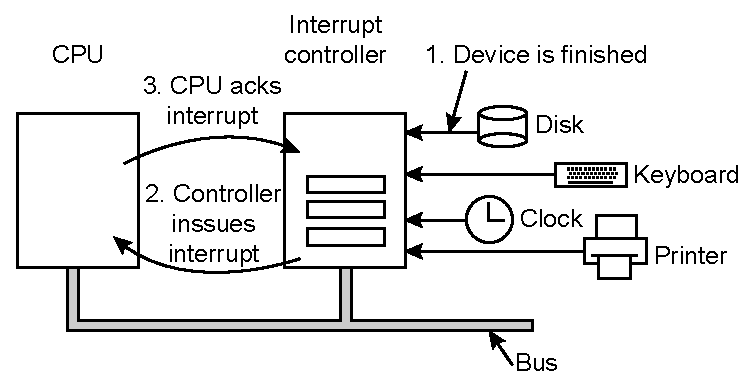
\includegraphics[width=\linewidth]{img/int.pdf}
	\caption{How an interrupt happens. The connections between the devices and the interrupt controller actually use interrupt lines on the bus rather than dedicated wires.}
\end{figure}

An interrupt that leaves the machine in a well-defined state is called a \textbf{precise interrupt}. Such an interrupt has four properties:
\begin{enumerate}
\item{The program counter (PC) is saved in a known place.}
\item{All instructions before the one pointed to by the PC have fully executed.}
\item{No instruction beyond the one pointed to by the PC has been executed.}
\item{The execution state of the instruction pointed to by the PC is known.}
\end{enumerate}

\section{Exercises}
Here follows some Q\&A.

\subsection{Q\&A - OS}
\paragraph{What is main tasks of bootstrap and BIOS?}
BIOS initialize hardware and checks if everything is OK. If it is, the rest of the software runs through reading the MBR on the first drive, and run the software on it (bootloader). The bootloader loads the operative system from disk and onto memory, and then run it.

\paragraph{What is user and kernel mode, and why cannot everything run in kernel mode?}
User mode: 
\begin{itemize}
\item{Ordinary software runs on this level.}
\item{Protected memory (a process cannot see memory used by other processes).}
\item{No access to hardware without using a system call.}
\end{itemize}

Kernel mode:
\begin{itemize}
\item{Only parts of the OS runs on this level. The software you can trust.}
\item{The software may do as they wish with the memory (even other processes), hardware, etc.}
\end{itemize}

When we do a system call from user mode, we will enter kernel mode, and the kernel will treat the request. 

\paragraph{What is the advantages and disadvantages with monolithic cores vs. micro-kernels?}
Monolithic:
\begin{itemize}
\item{Advantages: they are fast.}
\item{Disadvantage: difficult to maintain, may be unstable.}
\end{itemize}

Micro:
\begin{itemize}
\item{Advantages: easier to maintain and expand.}
\item{Disadvantage: slower.}
\end{itemize}

\paragraph{What is an interrupt, and what happens when one occur?}
Interrupts is a signal that signifies something unexpected occurred. For example when reading from disk, an interrupt may occur before it is done. The OS handle this signals.

When a interrupt occur, either by hardware or software, it will be sent to the kernel who puts a number on it. Then the kernel will run the function to that specific interrupt (number).

\subsection{Q\&A - Processes}
\paragraph{Why is program relocation unnecessary when we use virtual memory?}
This is unnecessary when a program is in a location which is different from the location that was made during the compiling. In virtual memory, all addresses is logical, not physic. 

\paragraph{In malware you will find this code at several locations: \texttt{if (fork() > 0) exit(0);} What happens?}
This code clones a child process while it is there. The result is the process changes PID, something that makes it hard to discover the program and have it killed.

\subsection{Q\&A - Processes}



\end{document}